\documentclass[14pt]{beamer}

\geometry{paperwidth=2in,paperheight=2in}

\usepackage{xcolor}
\usepackage{tikz}
\usepackage{ulem}

\setbeamercolor{background canvas}{bg=black}
\setbeamercolor{normal text}{fg=white}

\usetikzlibrary{positioning, shapes}
\usetikzlibrary{decorations.pathmorphing}

\setbeamertemplate{navigation symbols}{}
\setbeamersize{text margin left=0mm} 
\setbeamersize{text margin right=0mm} 

\setbeamertemplate{sidebar right}{default}{}

\begin{document}






\begin{frame}\Large
  \begin{center}
    Math is not a spectator sport.
  \end{center}
\end{frame}

\begin{frame}\Large
  \begin{center}
    Math is \textcolor{red}{\sout{not}} a spectator sport.
  \end{center}
\end{frame}

\begin{frame}\Large
  \begin{center}
    \textcolor{red}{WHY?} 
  \end{center}
\end{frame}

\begin{frame}\Large
  \begin{center}
\makebox[\paperwidth]{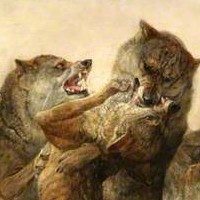
\includegraphics[width=\paperwidth]{struggle.jpg}}
  \end{center}
\end{frame}


\begin{frame}\Large
  \begin{center}
    Normalize failure
  \end{center}
\end{frame}

\begin{frame}\Large
  \begin{center}
    Own path
  \end{center}
\end{frame}


\begin{frame}\Large
  \begin{center}
    It's a journey
  \end{center}
\end{frame}

\begin{frame}\Large
  \begin{center}
    Lots of games
  \end{center}
\end{frame}


\begin{frame}\Large
  \begin{center}
    Share them with friends
  \end{center}
\end{frame}

\begin{frame}\Large
  \begin{center}
    Share them with enemies
  \end{center}
\end{frame}

\begin{frame}\Large
  \begin{center}
  Enemies become friends
  \end{center}
\end{frame}

\begin{frame}\Large
  \begin{center}
    THE END
  \end{center}
\end{frame}

\end{document}
